\chapter{Implementation}
\section{Database} \label{Database}
\begin{figure}[h]
\centering
\frame{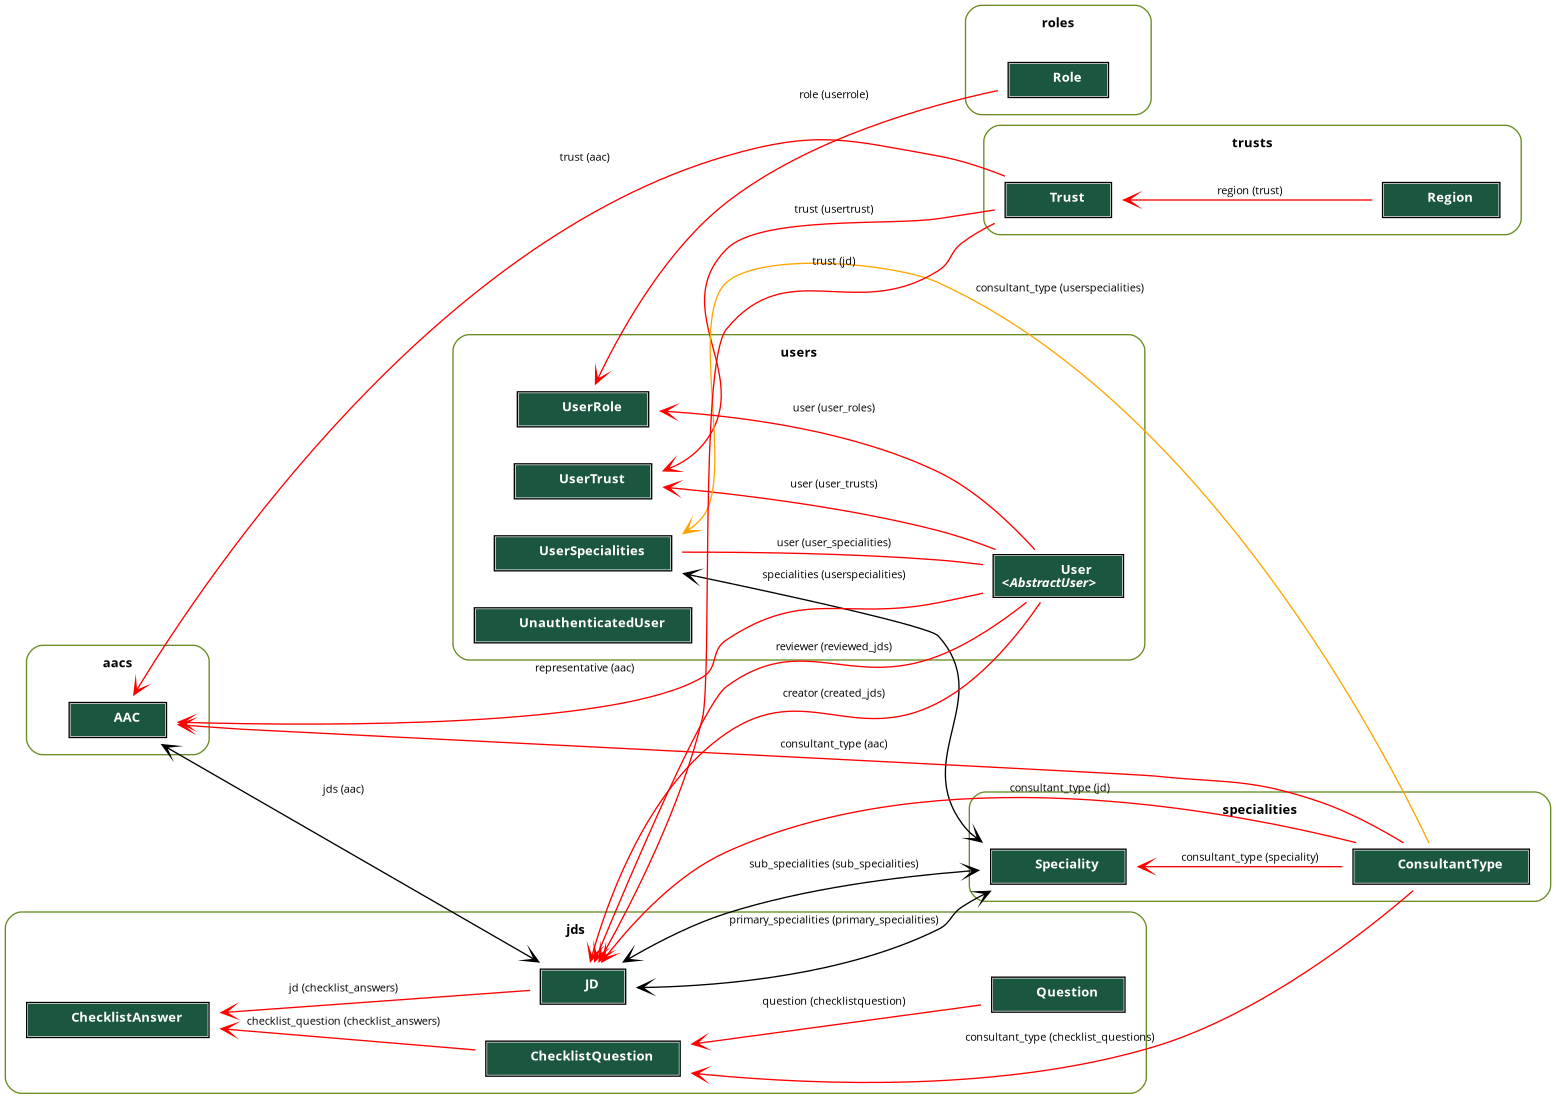
\includegraphics[width=\linewidth]{images/database.png}}
\vspace{-20pt}
\caption{The Database Schema without fields}
\label{fig:database}
\end{figure}
\vspace{-5pt}
Figure \ref{fig:database} represents the database schema. Due to the large number of models, fields have been omitted in this figure to maintain readability. See Appendix \ref{app:Database} for a full version. This diagram aptly presents just how intertwined this system is, as well as the sheet number of data taken into consideration during the process.

This relational database schema allows for handing of detailed user profiles, Job Descriptions (JDs), and Advisory Appointment Committees (AACs). It allows for a sophisticated access control system based on roles, Trust, and consultant types. The abundant use of foreign keys for relationships shows the normalisation practices taken to avoid data redundancy.

This schema allows handling detailed user profiles, job descriptions, and associated evaluations. It allows for a sophisticated access control system based on roles, trust levels, and consultant types, all of which can be tailored to the specific needs of an organization or system. The database schema utilizes foreign keys for relationships, suggesting it’s a relational database, and employs typical normalization practices to avoid data redundancy.

Normalization: The database avoids redundancy by normalizing data. Normalization helps in organizing data efficiently and reduces the redundancy by ensuring that each data item is stored only once. For instance, separating user details from roles and trust levels allows for easy updates and management of each aspect without unnecessary duplication.
Clarity in Relationships: The clear definition of relationships between entities, like one-to-many and many-to-many, indicates thoughtful consideration of how different data points relate to each other. This clarity supports accurate and efficient querying of the database.
Use of Abstract Entities: The use of an AbstractUser entity suggests an object-oriented approach to database design. This can make it easier to extend the database in the future because common attributes are centralized in the abstract entity.
Flexibility in Role Management: The separation of UserRole, UserTrust, and UserSpecialities allows for a flexible permission and access control system. It can handle complex scenarios where users can have multiple roles, varying levels of trust, and multiple specialties.
Hierarchical Specialization: The categorization of specialties into primary and sub-specialties indicates a hierarchical approach. This is beneficial for complex systems where specialties need to be organized in a detailed and hierarchical manner.
Modularity: The schema seems to be modular, as indicated by the presence of separate entities like aacs and jds. This modularity allows for distinct parts of the application to evolve independently and makes the system easier to maintain.
Data Integrity: The schema likely enforces data integrity through the use of foreign keys which ensure that relationships between entities are consistent and that orphan records are avoided.
Comprehensive Data Capture: Entities have attributes that capture a broad range of data points, from user information to job descriptions, which would enable detailed analysis and reporting.
Scalability: With its structured approach to data separation and relationships, the schema allows for scalability. As the system grows and the amount of data increases, such a schema can handle the growth without major changes.
Security Considerations: By separating UnauthenticatedUser and User, the schema indicates a focus on security, allowing the system to differentiate between verified and unverified users.
Regional Specificity: The inclusion of Region in the Trust entity allows the database to cater to regional variations in data, which can be crucial for businesses operating in multiple jurisdictions.
Timestamps for Tracking Changes: Entities like User and JD contain timestamps, which are essential for tracking changes over time and for audit purposes.



\section{app.pcss}

\newpage
\section{REDO THIS}
\section{Django}
\subfile{implementation/database}
\subsection{Schemas}
pydantic
\subsection{Services}
django
\subsection{API Endpoints}
django-ninja \& django-ninja-jwt

\section{SvelteKit}
\subfile{implementation/design}

\subsection{API Consumption}

\subfile{implementation/auth}

\subfile{implementation/profile}

\subfile{implementation/panel}